\section{Motivation}

The advancement of technology has brought about new computing paradigms and network technologies that have the potential to revolutionize the way we think about and approach computing and communication.
One of the most promising of these is Edge Computing, a distributed computing paradigm which seeks to bring compute nodes closer to the end user, reducing latency (i.e.\ the time between input and response) and increasing reliability.

The current model for distributed computing, known as Cloud Computing, allows users to access shared pools of resources, services, and applications over the internet~\cite{gai2012towards}.
Cloud computing offers many advantages, including as virtually unlimited storage and processing power.
This is achieved by virtue of employing economies of scale in massive installations containing up to thousands of compute servers and networking equipment.
These installations are known as \emph{datacenters}, and often serve massive amounts of users.

However, this design leads to trade-offs in bandwidth and, particularly, latency.
Cloud datacenter are commonly located in geographically centralized locations to better serve thousands or even millions of users.
Conversely, this results in these datacenters having a large average \emph{topological} and \emph{physical} distance to individual users.
Topologically, end-user connections to the Cloud tend to transit a significant number of hops, i.e.\ intermediate connections through networking equipment belonging to service providers at multiple tiers of the internet.
Data needs to be received, routed, and re-transmitted at each hop, adding delay.
Physically, Cloud datacenters are often located hundreds or even thousands of kilometers from end-users.
Connections are limited in their responsiveness by the speed of light, and long physical distances directly translate into higher latencies.

These limitations of the Cloud make it unsuitable for a number of novel applications that require quick response times, such as real-time video processing, \gls{MAR}, or smart city systems.
Additionally, the centralized nature of Cloud datacenters means that it can be vulnerable to outages or other disruptions, which can impact large numbers of users simultaneously.

\begin{figure}
    \centering
    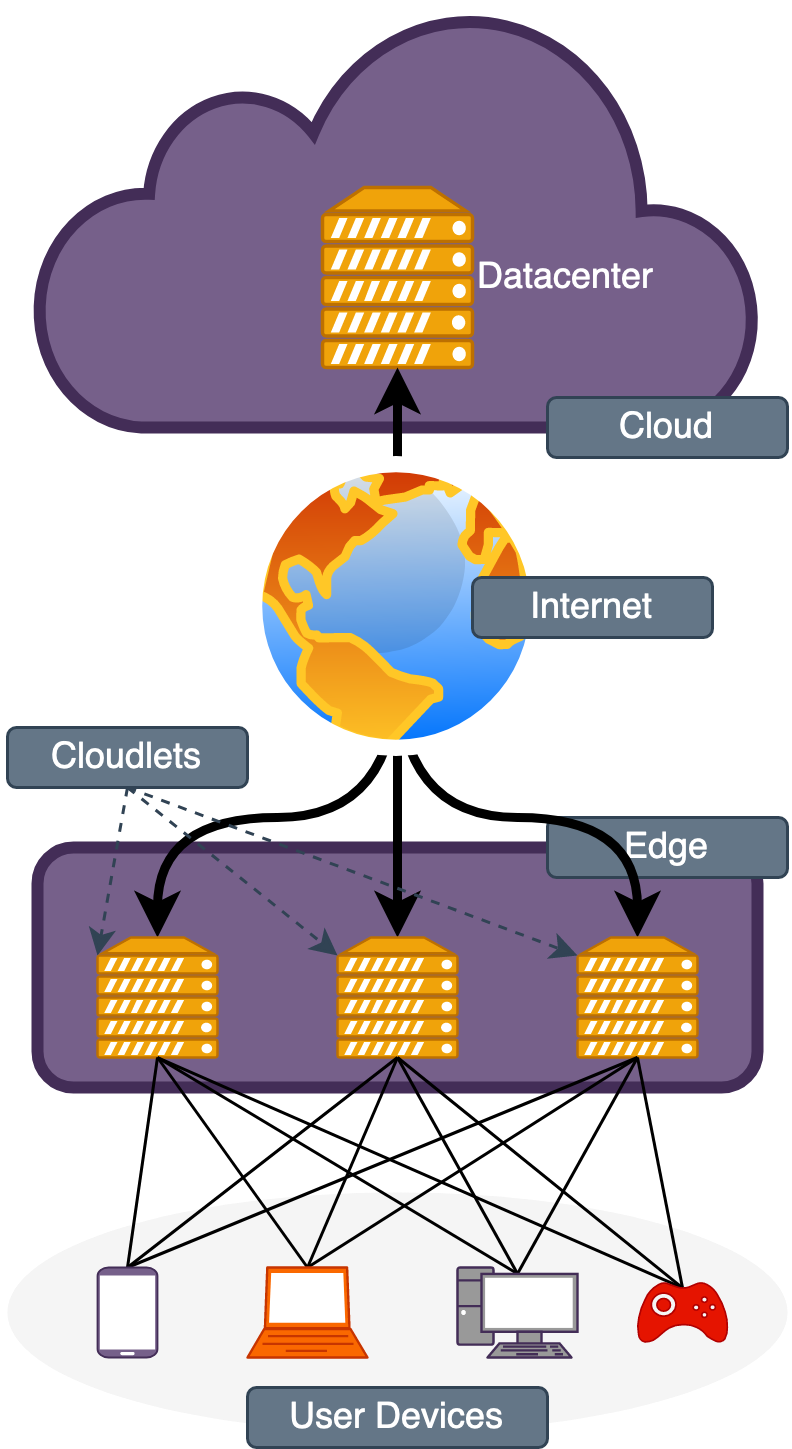
\includegraphics[height=30em]{figures/edgecomputing}
    \caption{%
        Conceptual design of Edge Computing.
        Compute nodes are placed a at the edge of the network, a few hops away from end users.
        In other words, compute is located between users and the internet and the Cloud.
    }\label{fig:edgecomputing}
\end{figure}

Edge Computing aims to improve upon the shortcomings of Cloud Computing by moving the processing closer to the end user, at the \emph{edge} of the network.
In this context, the ``edge of the network'' refers to locations which are both geographically and topologically close to the user, such as micro-datacenters located within the same urban area as the user (see \cref{fig:edgecomputing}).
\gls{MEC}, a variant of the paradigm, even proposes the integration of compute power within 5G~\cite{5Gstandard} cellular networks, co-locating computed nodes with cellular service provider base stations.

By placing computing resources in proximity to where data is generated and/or consumed, and thus reducing the topological and physical distances that data must travel, Edge Computing can greatly decrease latency, improve the responsiveness of applications, and allow for greatly improved efficiency in the use of network resources.
This enables powerful and sophisticated applications to be run on the Edge, such as \glspl{CPS} as well as \gls{XR} applications.
These applications have the potential to cause a profound impact in our day-to-day lives, but have stringent latency requirements which make their deployment on traditional paradigms such as Cloud Computing inviable.

\glspl{CPS} refers to systems where physical processes, such as manufacturing or transportation, are controlled  and monitored by computers, usually over communication networks.
Edge Computing allows these systems to operate in real-time, enabling near instantaneous response times, more efficient operation, and more precise control.
These characteristics are critical for applications such as \glspl{ITS}, autonomous driving, or remote surgery.

\gls{XR}, on the other hand, is a broad term that encompasses various forms of immersive applications.
\gls{XR} applications, such as \gls{AR}, \gls{VR}, or \gls{MR}, involve the real-time interaction between user and virtual elements in a partially to fully immersive environment.
For instance, \gls{MAR} is an application of \gls{AR} that involves overlaying digital information onto the physical world using a mobile device.
This definition has in later years been extended to encompass \gls{AR} deployed on wearable devices (such as Google Glass~\cite{googleglass}).
\gls{MAR} allows users to, for example, view real-time information and details about products while in-store, receive instructions and guidance to perform a complex task, or contextual information while visiting a new city.
An  example of such an application is illustrated in \cref{fig:augmentedreality}.
By using Edge Computing and 5G, \gls{MAR} --- and other \gls{XR} systems --- can operate with much greater responsiveness and reliability, enabling highly immersive and interactive experiences.

\begin{figure}
    \centering
    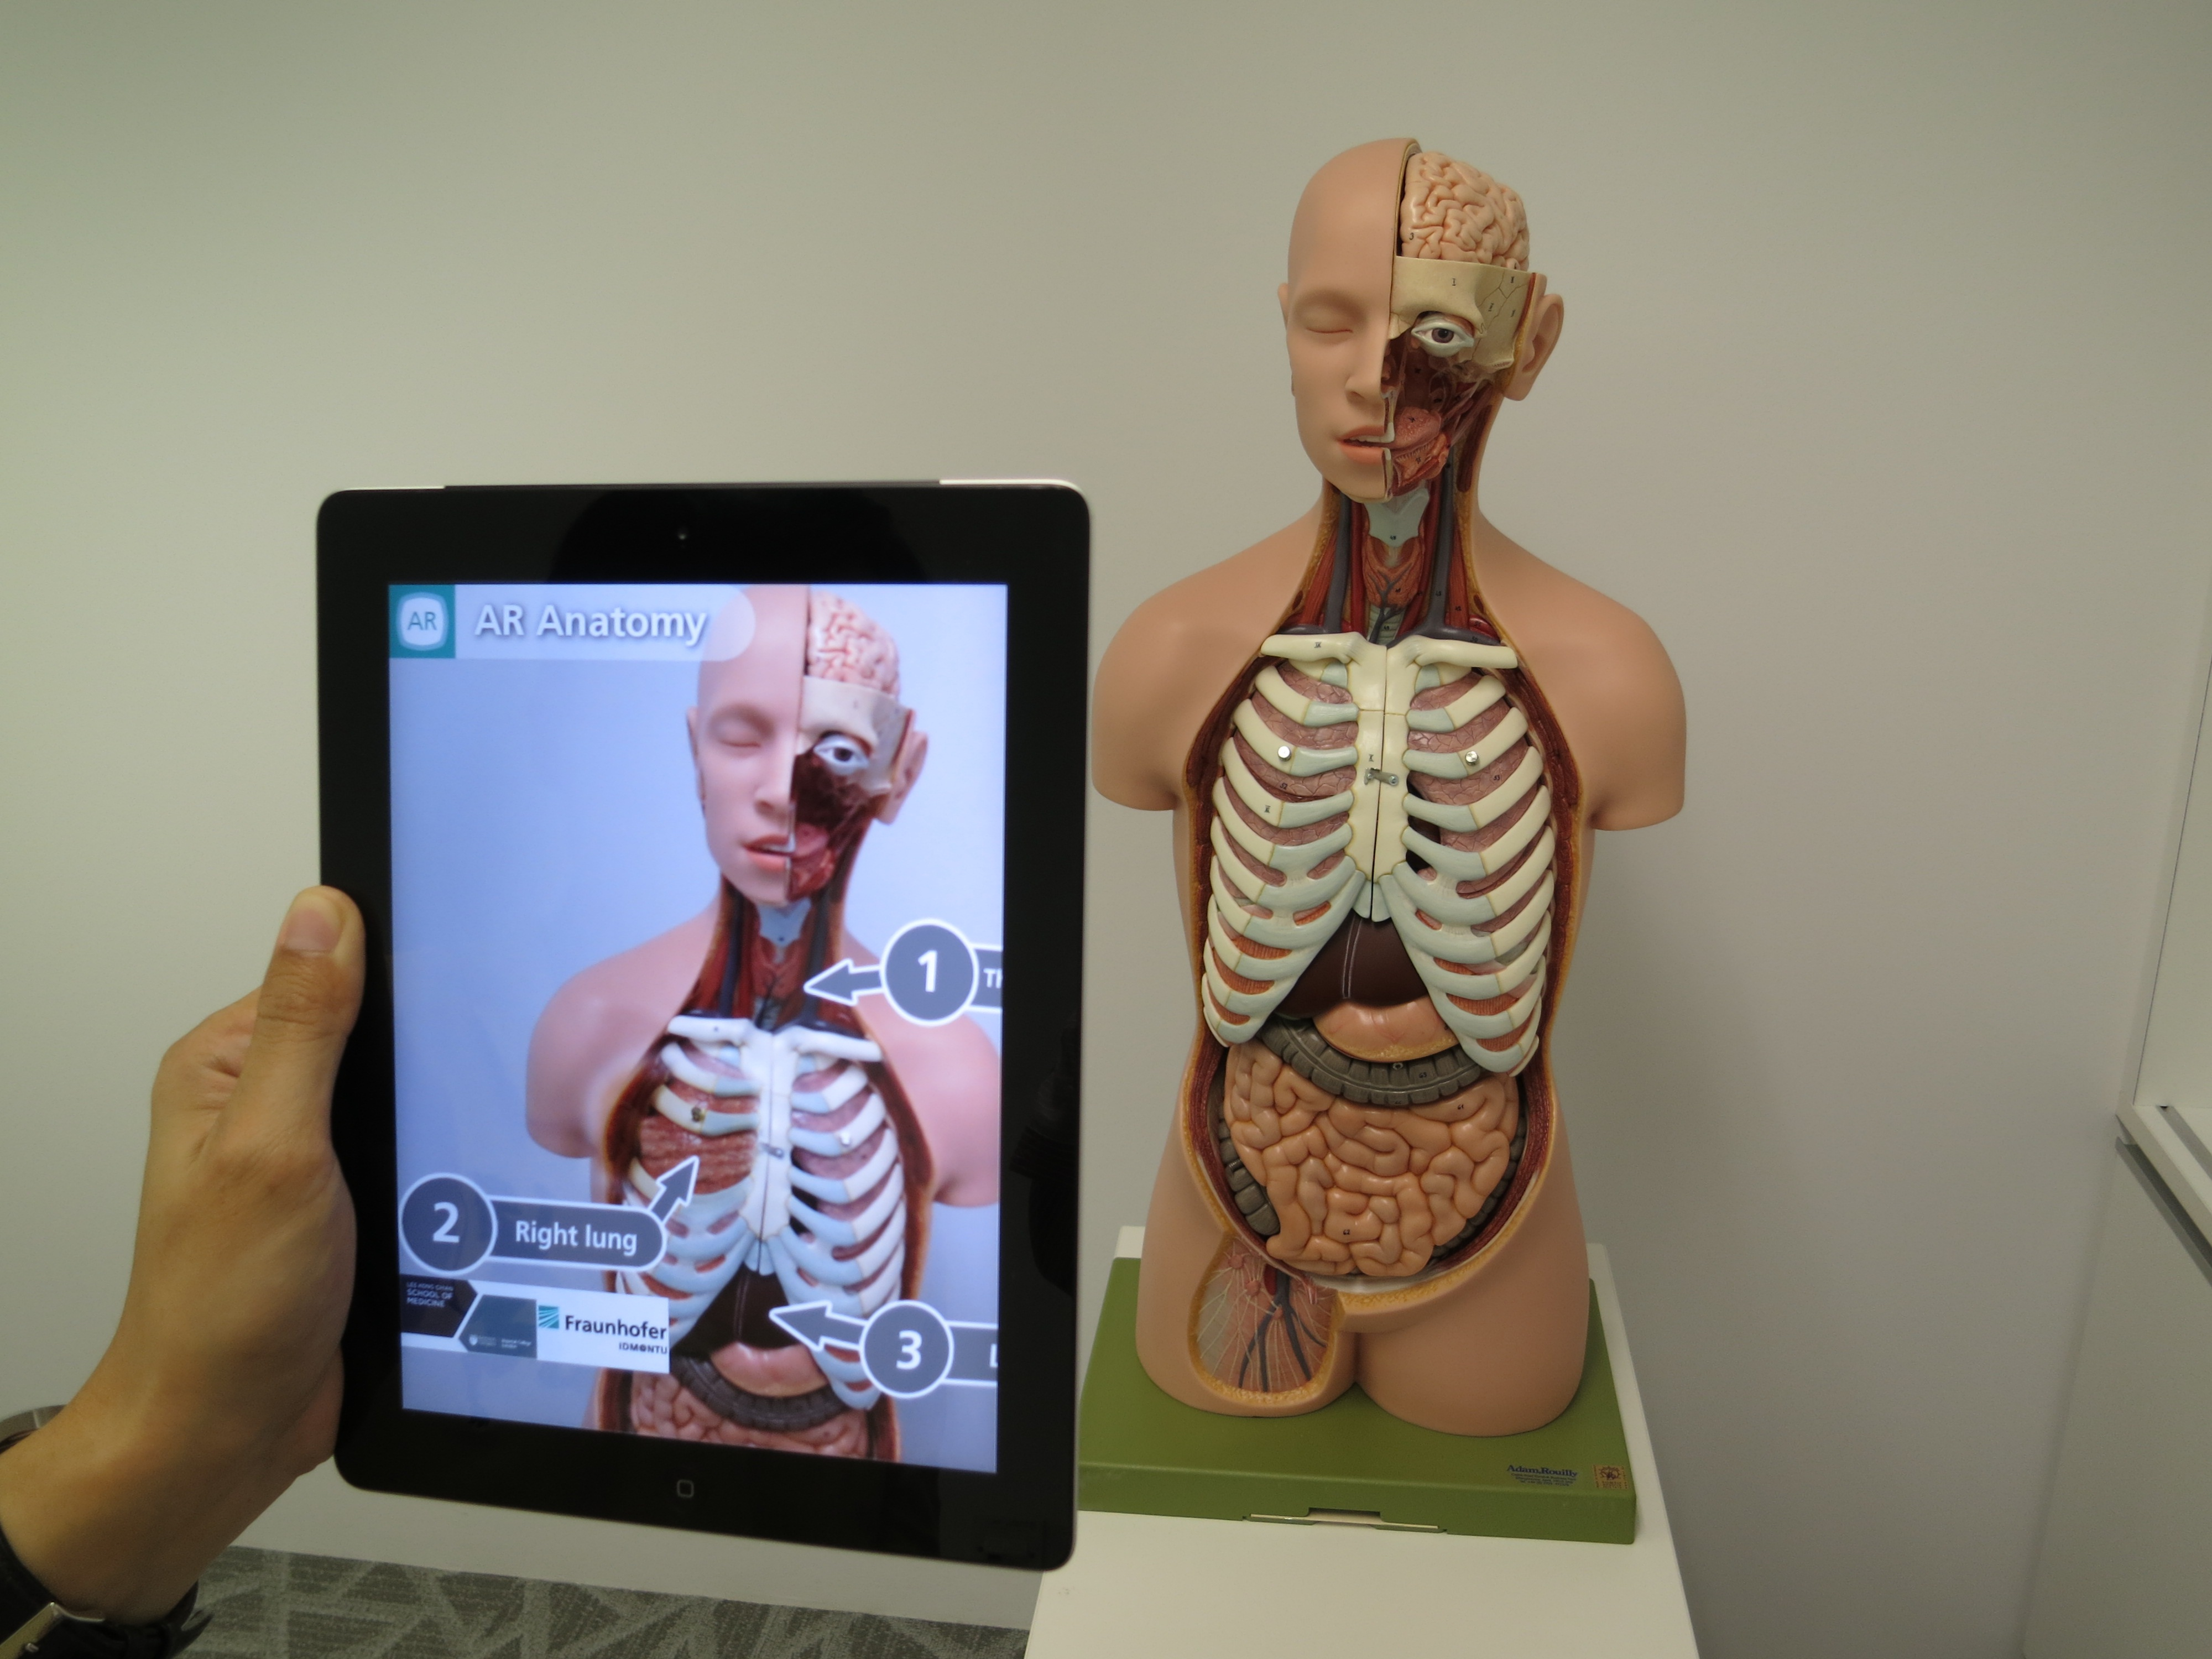
\includegraphics[height=26em]{figures/AR}
    \caption[{ }]{
        Example of an \gls{AR} application that overlays anatomical information on top of a live video feed of a model of human anatomy.\\
    
        {
            \footnotesize%
            Photo source: Pixabay~\cite{picture:AR}.
            Licensed under a \gls{CC0} license.
        }
    }\label{fig:augmentedreality}
\end{figure}

Overall, the combination of Edge Computing and 5G holds great promise for the massive deployment of latency-sensitive applications such as the ones discussed above.
Nonetheless, significant challenges remain in the understanding and scaling of these systems, particularly in regard to their complexity and requirements in the context of low-latency, high-reliability computing.

Before widespread deployment of these systems, it is crucial to thoroughly understand their real-world performance.
\glspl{CPS} often correspond to safety-critical components of industrial systems, and subpar \gls{QoS} can therefore lead to significant danger to equipment and operators.
On the other hand, the immersive nature of \gls{XR} applications implies that poor \gls{QoS} can easily translate into significant user discomfort.
To ensure reliability, safety, and user satisfaction in these systems, careful and accurate characterization and optimization of these systems must be realized.

However, evaluating the performance of such applications on Edge environments represents a significant challenge.
Latency-sensitive applications such as \glspl{CPS} and \gls{XR}, involve multiple processing steps that can influence the latency of the system.
There are many trade-offs involved in optimizing the latency of these applications beyond the question of where the compute process is located. 
These include the choice of wireless system for transmitting application data (e.g.\ 4G \gls{LTE} versus 5G), the protocols used to communicate over the network, and the hardware and operating system used in the backend.
In the case of \gls{XR}, the sensory inputs need to be pre-processed and compressed on-device, before being transmitted to the compute backend for processing.
The backend algorithms need to be carefully designed and implemented to ensure efficient processing and minimal latency. 
Similarly, in \glspl{CPS}, the communication network must be designed to minimize latency and ensure reliable data transmission between the components of the control system.
Other critical aspects with the potential to impact the latency of latency-sensitive applications on the Edge include congestion on the communication loop and fluctuations of the wireless channel.
These issues can lead to delays in data transmission between devices on the network, leading to higher end-to-end latency.

The evaluation of performance in Edge Computing has been addressed in existing works through analytical~\cite{chen2015efficient,champati2015one,champati2016semi,al2017reliable}, simulation~\cite{svorobej2019simulating,gupta2017ifogsim,sonmez2018edgecloudsim,qayyum2018fognetsimpp}, and experimental~\cite{das2018edgebench,lee2019iotbench,george2020openrtist,mcchesney2019defog,baurle2022comb} approaches.
However, these systems exhibit characteristic that make their study complex.
One of these is the unique nature of Edge computing environments, which tightly integrates compute and network.
This demands a wide range of interdisciplinary expertise to study, spanning (but not limited to) computer science, communication networks, information theory, and queuing analysis.
Such expertise may not always be feasible to obtain within a single research group.

The highly complex effects emerging from the interaction between network and compute is another major hurdle to studying latency-sensitive applications on Edge Computing.
These effects are specially difficult to address through analytical models and simulations, particularly in multi-tenant deployments, where each tenant may have different requirements and resource usage patterns.
Although powerful approaches to the modeling of network effects and compute process scheduling exist in literature, existing analytical and simulation approaches have so far not managed to combine the two.

Nevertheless, experimental approaches also face important challenges.
One of these stems from the fact that latency-sensitive applications such as \gls{CPS} and \gls{XR} on Edge Computing interact with the real world.
This implies that these applications thus must be studied in real-time to achieve comprehensive characterization.
Thus, any study of these applications must be done in an environment that accurately reflects the real-world conditions in which they are deployed.
Unfortunately, replicating these conditions in a controlled experimental environment is difficult and often leads to inconsistencies in results, and traditional methods that rely on simulations may not be sufficient to accurately capture and evaluate the performance of these applications in real-world scenarios.

The scalability of these systems is also a challenge.
It may not be feasible for researchers to test the applications on a large scale due to limitations in access to specialized equipment, test subjects, as well as facilities.
\glspl{CPS} often rely on physical sensors and actuators, making it difficult to replicate real-world conditions in a controlled environment at scale, and conducting experiments involving human subjects for \gls{XR} is time-consuming and expensive.
This also makes the study of these applications hard to automate, making it challenging to conduct large-scale experiments or to collect data over an extended period of time.

This has led to existing approaches to performance evaluation of Edge Computing environments to often be constrained in their scope, focusing on comprehensive characterization of either compute or network aspects (e.g.~\cite{chen2015efficient} and~\cite{al2017reliable}), resulting in potential trade-offs that may neglect one half of the larger picture.
I argue that this limitation has led to an incomplete understanding of the overall performance of Edge systems and applications in the existing literature.
There is a need for holistic approaches that consider both network and compute characteristics of Edge workloads for accurate performance evaluation and optimization.

This dissertation aims to contribute to the field by presenting two key contributions.
First, I introduce and subsequently investigate the applications of a methodology for the study of latency-sensitive applications deployed on Edge environments.
The proposed methodology is based on the emulation of workloads and aims to enhance the accuracy and realism of results related to Edge infrastructure and 5G networks, particularly in regard to network performance.
Next, I present a deeper exploration of the implications of improved accuracy in the emulated components of my methodology by studying potential avenues for optimization of a particular sub-class of \gls{MAR}.

My methodology is designed to tackle these challenges by employing an emulation approach to the benchmarking of latency-sensitive \gls{CPS} and \gls{XR} applications. 
I emulate target workloads on actual Edge infrastructure by replacing the client side of the system with \gls{COTS} general-purpose computing devices\footnote{%
    In my initial implementation, these correspond to low-cost and easily replaceable, scalable Raspberry Pi 4 Model B \acsp{SBC}.
} running a realistic software imitation of the desired behaviors.
At the same time, my methodology retains the real network as well as the real compute hardware and software at the backend.
This design results in real-time benchmarking and performance evaluation of applications and Edge infrastructure, while still providing realism, scalability, and reduced complexity, as well as allowing for easier automation of these studies.

Emulating the workload component reduces complexity by moving it into the software domain, allowing for improved repeatability and replicability, as well as easier horizontal scaling through the use of \gls{COTS} general-purpose hardware such as \glspl{SBC}.
This also reduces the barrier of entry to this research, as \glspl{SBC} are for the most part cheap and easily accessible.
Additionally, it preserves the realism of effects stemming from the hardware and network.
In particular, the methodology allows for the capture of effects due to the interaction of network factors such as contention, congestion control, and medium access, with factors due to process scheduling and/or resource contention at the compute level.
These effects are often of stochastic or chaotic natures and complex to capture in models or simulations.

Next, I study how improved accuracy in the emulations employed by this methodology can open new avenues for the optimization of applications on Edge Computing.
To achieve this, I develop a model for human behavior in a subclass of \gls{MAR} which is able to dynamically adapt to changes in system responsiveness.
I combine it with a mathematical framework to study the potential for optimization of resource consumption in these applications, and find that improved accuracy in the emulation enables otherwise inviable optimization approaches.

I believe my contributions represent valuable tools and insights for researchers, system designers, and application developers.
The methodology represents a novel, holistic approach to the performance evaluation of Edge environments.
Furthermore, my findings have significant implications for the design and optimization of applications enabled by Edge Computing, particularly in the areas of energy consumption, sampling strategies, and application lifetime.
I hope and believe this dissertation will contribute to the development of new techniques and approaches for improving the performance and reliability of Edge Computing.